% Nishant D. Gurnani
% A Case Study on Model-Free Volatility Prediction
% MATH 289A - Topics on the Bootstrap & Subsampling

% FORMATTED FOR THESIS BINDING
\documentclass[11pt,]{article}
\usepackage[top=1in, left=1in, right=1in, bottom=1in]{geometry}

\usepackage{geometry}
\usepackage{amsmath,amssymb}
\usepackage{hyperref}

\makeatletter
\newcommand{\xRightarrow}[2][]{\ext@arrow 0359\Rightarrowfill@{#1}{#2}}
\makeatother

\geometry{letterpaper}

% For figures
\usepackage{graphicx} % more modern
\usepackage{subfigure} 
\usepackage{float}
\floatstyle{boxed}
\restylefloat{figure}

% For ceiling function
\usepackage{mathtools}
\DeclarePairedDelimiter{\ceil}{\lceil}{\rceil}


\newcommand{\id}{\mathrm{id}}
\newcommand{\K}{\mathrm{KL}}
\newcommand{\kl}{\mathrm{kl}}
\newcommand{\bp}{\boldsymbol{p}}
\renewcommand{\phi}{\varphi}
\renewcommand{\a}{\alpha}

\renewcommand{\P}{\mathbb{P}}
\newcommand{\E}{\mathbb{E}}
\newcommand{\N}{\mathbb{N}}
\newcommand{\R}{\mathbb{R}}
\newcommand{\Q}{\mathbb{Q}}
\newcommand{\KL}{\mathrm{KL}}
\newcommand{\LG}{\overline{\log}(d)}
\newcommand{\LGG}{\overline{\log}(M K)}
\newcommand{\ocP}{\overline{\mathcal{P}}}

\newcommand{\cO}{\mathcal{O}}
\newcommand{\cZ}{\mathcal{Z}}
\newcommand{\cA}{\mathcal{A}}
\newcommand{\cB}{\mathcal{B}}
\newcommand{\cN}{\mathcal{N}}
\newcommand{\cM}{\mathcal{M}}
\newcommand{\cF}{\mathcal{F}}
\newcommand{\cL}{\mathcal{L}}
\newcommand{\cX}{\mathcal{X}}
\newcommand{\cI}{\mathcal{I}}
\newcommand{\cJ}{\mathcal{J}}
\newcommand{\cY}{\mathcal{Y}}
\newcommand{\cH}{\mathcal{H}}
\newcommand{\cP}{\mathcal{P}}
\newcommand{\cT}{\mathcal{T}}
\newcommand{\cC}{\mathcal{C}}
\newcommand{\cS}{\mathcal{S}}
\newcommand{\cE}{\mathcal{E}}
\newcommand{\cK}{\mathcal{K}}
\newcommand{\cD}{\mathcal{D}}

\newcommand{\oD}{\overline{\mathcal{D}}}
\newcommand{\oR}{\overline{R}}

\def\ds1{\mathds{1}}
\renewcommand{\epsilon}{\varepsilon}

\newcommand{\wh}{\widehat}
\newcommand{\argmax}{\mathop{\mathrm{argmax}}}
\newcommand{\argmin}{\mathop{\mathrm{argmin}}}
\renewcommand{\mod}[2]{[#1 \,\, \mathrm{mod} \,\, #2]}
\newcommand{\todo}{{\bf TO DO } }

\renewcommand{\tilde}{\widetilde}

%Cadres d'algorithmes
\newlength{\minipagewidth}
\setlength{\minipagewidth}{\columnwidth}
\setlength{\fboxsep}{3mm}
\addtolength{\minipagewidth}{-\fboxrule}
\addtolength{\minipagewidth}{-\fboxrule}
\addtolength{\minipagewidth}{-\fboxsep}
\addtolength{\minipagewidth}{-\fboxsep}
\newcommand{\bookbox}[1]{\small
\par\medskip\noindent
\framebox[\columnwidth]{
\begin{minipage}{\minipagewidth} {#1} \end{minipage} } \par\medskip }

%%
%

\newcommand{\Ber}{\mathop{\mathrm{Ber}}}

\newcommand{\beq}{\begin{equation}}
\newcommand{\eeq}{\end{equation}}

\newcommand{\beqa}{\begin{eqnarray}}
\newcommand{\eeqa}{\end{eqnarray}}

\newcommand{\beqan}{\begin{eqnarray*}}
\newcommand{\eeqan}{\end{eqnarray*}}

\def\ba#1\ea{\begin{align*}#1\end{align*}} %\ba = \begin{algin*}, \ea = \end{align*}
\def\banum#1\eanum{\begin{align}#1\end{align}} %\banum = \begin{algin}, \eanum

%\newcommand{\qed}{\hfill\BlackBox}
\newcommand{\charfct}{\ds1} %
\newcommand{\Fcal}{\mathcal{F}}
\newcommand{\Xcal}{\mathcal{X}}
\newcommand{\Hcal}{\mathcal{H}}
\newcommand{\Gcal}{\mathcal{G}}
\newcommand{\Nat}{\mathbb{N}}




% For citations
\usepackage{natbib}

% For algorithms
\usepackage{algorithm}
\usepackage{algorithmic}

\newcommand{\skipline}{\vspace{12pt}}
\newtheorem{thm}{Theorem}[section]
\newtheorem{lemma}[thm]{Lemma}
\newtheorem{prop}[thm]{Proposition}
\newtheorem{defn}[thm]{Definition}





\title{A Case Study on Model-Free Volatility Prediction in Financial Time Series}
\author{Nishant D. Gurnani \\ \\ MATH 289A - Topics on the Bootstrap \& Subsampling}

%The well-known ARCH/GARCH models for financial time series have been criticized for their poor performance in volatility prediction, i.e., prediction of squared returns. Focusing on three representative data series, namely a foreign exchange series (Yen vs. Dollar), a stock index series (the S&P500 index), and a stock price series (IBM), the case is made that financial returns may not possess a finite fourth moment. Taking this into account, we show how and why ARCH/GARCH models—when properly applied and evaluated—actually do have nontrivial predictive validity for volatility. Furthermore, we show how a simple model-free variation on the ARCH theme can perform even better in that respect. The model-free approach is based on a novel normalizing and variance–stabilizing transformation (NoVaS, for short) that can be seen as an alternative to parametric modeling. Properties of this transformation are discussed, and practical algorithms for optimizing it are given.

%\pagestyle{headings}

\begin{document}
\maketitle


\section{Introduction} \label{sec:intro}

Volatility clustering in financial times series is the phenomena first observed in Mandelbrot (1963) \cite{Mandelbrot1963} that ``large changes tend to be followed by large changes, of either sign, and small changes tend to be followed by small changes." The clustering of days with high volatility and similarly days with low volatility is a counter-intuitive statistical property of financial time series data that manifests itself  across all asset classes. Consequently, volatility prediction forms the foundation of a number of quantitative investment strategies (such as volatility arbitrage where the objective is to take advantage of differences between the implied volatility of an option, and a forecast of future realized volatility of the option's underlying) and is instrumental in the construction of sound risk models. %The literature on volatility prediction is quite large and we refer the interested reader to Poon and Granger (2003) \cite{PoonGranger2003} and Andersen et. al (2006) \cite{Andersen2006} for comprehensive reviews of the subject.

The celebrated Autoregressive Conditional Heteroscedasticity (ARCH) models of Engle (1982) \cite{Engle1982} and Generalized Autoregressive Conditional Heteroscedasticity (GARCH) models of Bollerslev (1986) \cite{Bollerslev1986} were designed to capture the phenomenon of volatility clustering by postulating a particular structure of dependence for the time series of squared returns. Despite their popularity, the simple and neat parametric formulation of the models cannot be expected to perfectly capture the behavior of complicated real-world phenomenon such as the evolution of financial returns. This is observed empirically in the fact that the models are able to only partially account for the heavy tails empirically found in the distribution of returns. Consequently, as a more realistic alternative we consider the model-free prediction of approach of Politis (2007) \cite{Politis2007} in trying to understand this complex type of data.

In this project, we explore the performance of the model-free paradigm in the context of volatility prediction. Our objective is to show that the model-free approach outperforms the ubiquitous GARCH model and we illustrate our results on daily returns of futures contracts. Our investigation closely follows Chapter 10 in Politis (2015) \cite{Politis2015}.

\section{Model-Based Prediction} \label{sec:garch}

Model-based methods are ubiquitous in statistics and the current dominant prediction paradigm involves first constructing/fitting a model, and then using the fitted model for prediction. For volatility prediction, we consider the problem of prediction of $Y_{n+1}^2$ based on the observed past $F_n = \{Y_t, 1\leq t \leq n \}$.

\subsection{Simple Forecasting Methods}

Under the common assumption that the return series $\{Y_t\}$ is strictly stationary with mean zero, we can define a naive predictor as the empirical estimate of the (unconditional variance) $\sigma_{y}^2$ of the series $\{Y_t, 1\leq t \leq n \}$. As a result, we define our baseline predictor as follows: 

\begin{equation}
s_{n}^2 = \frac{1}{n} \sum_{k=1}^{n} Y_{k}^2
\end{equation}

As an immediate improvement over our naive benchmark above, we can also consider the simple exponential smoothing forecasting method (see Hamilton (1994) \cite{Hamilton1994}). The exponential smoothing predictor of $Y_{n+1}^2$ is of the form:

\begin{equation}
\frac{\sum_{k=1}^{q} \delta^k Y_{n-k}^2}{\sum_{j=1}^{q}\delta^j}
\end{equation}

where $\delta \in (0,1)$ and $q$ is an appropriate practical truncation limit.

\subsection{ARCH/GARCH Models}

Finally we consider the ARCH/GARCH models, which by their very design, attempt to capture the phenomenon of volatility clustering in a simple equation. A typical ARCH($p$) model is described by an equation of the type:

\begin{equation}
Y_t = Z_t \sqrtsign{a + \sum_{i=1}^p a_i Y_{t-i}^2}
\end{equation}

where the series $\{Z_t\}$ is assumed to be i.i.d. $N(0,1)$ and $p$ is an integer indicating the order of the model.

The ARCH model is a generalization of the sample variance. That is, instead of giving equal weight to each residual squared observed across time, you estimate what weights to give each using historical data and a procedure such as maximum likelihood.

Following the methodology of Chapter 10 in Politis (2015) \cite{Politis2015}, we focus on the GARCH model. In particular, the GARCH(1,1) model is the most popular among the GARCH(p,q) models as it is believed to achieve the most parsimonious fit for financial returns data. The GARCH(1,1) model is described by the equation:

\begin{equation}
Y_t = h_t Z_t \hspace{0.5cm} \textnormal{with} \hspace{0.5cm} h_{t}^2 = C + AY_{t-1}^2 + Bh_{t-1}^2
\end{equation}

where the $\{Z_t\}'s$ are i.i.d. (0,1) and the parameters $A,B,C$ are assumed nonnegative. The quantity $h_{t}^2 = \E(Y_{t}^2|F_{t-1})$ is the volatility defined as $a + \sum_{i=1}^{p}a_iY_{n-i}^2$.

GARCH is similar to ARCH (it is easy to show that it is equivalent to the ARCH model with $p=\infty$) but employs a different weight scheme that can still be estimated, tested and then used to forecast volatility. Robert Engle, in his Nobel address \cite{EngleNobel}, uses the GARCH(1,1) model as an example to illustrate how one could interpret such a model. He says, ``the GARCH forecast variance is a weighted average of three different variance forecasts. One is a constant variance that corresponds to the long run average. The second is the forecast that was made in the previous period. The third is the new information that was not available when the previous forecast was made. This could be viewed as a variance forecast based on one period of information. The weights on these three forecasts determine how fast the variance changes with new information and how fast it reverts to the long run mean."

The ARCH/GARCH models are widely used in industry to forecast volatility and as such represent the main methods we wish to outperform with the model-free approach. Additionally, we note that as there is no closed-form solution for the maximizer of the models, the MLEs are found by numerical optimization which is not always stable unless the sample size is large.

\section{Model-Free Prediction Principle} \label{sec:modelfree}
Model-based prediction methods suffer from a number of disadvantages. The intermediate step of model-building/fitting can be problematic as it is always in a state of flux. The model that is settled on is not necessarily ``true", it's simply the model for which no apparent problems manifest. Additionally, optimal methods for model-fitting are not always robust. As mentioned above, the numerical optimization used to find the MLEs for the ARCH/GARCH models is not always stable and requires large sample sizes. Finally, nothing stops the practitioner from performing optimal prediction using the wrong model. Depending on the optimality criterion chosen for prediction it is entirely possible to fit a model that performs well with respect to the criterion but fails to accurately model the data.

The model-free prediction principle allows us to remove the intermediate step of model-fitting and perform prediction in a direct way. Consequently, model-free prediction removes the emphasis on parameter estimation and focuses on the observable quantities i.e. current and future data. The main idea of the model-free prediction principle is to use the structure of the problem to find an invertible transformation $H_m$ that can map the non-i.i.d. vector $Y_m$ to a vector $\underline{\epsilon_m} = (\epsilon_1, \dots, \epsilon_m)$ that has i.i.d components.

\begin{equation}
\underline{Y_m} \xrightarrow{H_m} \underline{\epsilon_m} \hspace{0.3cm} \text{and} \hspace{0.3cm} 
\underline{\epsilon_m} \xrightarrow{H_{m}^{-1}} \underline{Y_m}
\end{equation}

As a result, once the model-free procedure has been successfully implemented (i.e. a proper transformation $H_m$ is chosen) then the prediction problem is reduced to the simple one of predicting i.i.d variables. Finding the correct transformation is not always straightforward and the normalizing and variance-stabilizing transformation (NoVaS) which we use for volatility prediction uses the transformation to normality as a stepping-stone towards a transformation to ``i.i.d.-ness".

\subsection{Normalization and Variance Stabilization (NoVaS)}
We wish to find a transformation that will map the dataset $Y_1,\dots,Y_n$ to a Gaussian one. Our starting point is the ARCH model (3), under which the quantity

\begin{equation}
\frac{Y_t}{\sqrtsign{a + \sum_{i=1}^p a_i Y_{t-i}^2}}
\end{equation}

is assumed to be i.i.d $N(0,1)$ and hence is perfectly normalized and variance-stabilized. However, we note that there is no reason to exclude the value of $Y_t$ from an empirical, casual estimate (only involves past and present data) of the standard deviation of $Y_t$. Using this insight, the normalizing and variance-stabilizing transformation (NoVaS) is defined as

\begin{equation}
W_{t,a} \coloneqq \frac{Y_t}{\sqrtsign{\alpha s_{t-1}^2 + a_{0} Y_{t}^2 + \sum_{i=1}^p a_i Y_{t-i}^2}} \hspace{0.3cm} \text{for} \hspace{0.3cm} t = p+1, p+2, \dots, n; 
\end{equation}

where $s_{t-1}^2$ is an estimator of $\sigma_{Y}^2 = Var(Y_1)$ and the transformation maps the time series $\{Y_t\}$ to the new series $\{W_{t,a}\}$. The order $p \geq 0$ and the vector of nonnegative parameters $(\alpha, a_0, \dots, a_p)$ are chosen by the practitioner with the twin goals of normalization and variance stabilization.

\subsubsection{Choosing the Parameters of NoVaS}
Given the twin goals of normalization and variance stabilization, we impose certain constraints on the order $p \geq 0$ and the vector of nonnegative parameters $(\alpha, a_0, \dots, a_p)$ based on assumptions of the structure of the time series. We wish to construct a local estimator of scale for studentization purposes and thus require

\begin{equation}
\alpha \geq 0, a_i \geq 0 \hspace{0.3cm} \text{for all} \hspace{0.3cm} i \geq 0, \hspace{0.3cm} \text{and} \hspace{0.3cm} \alpha + \sum_{i=0}^{p} a_i = 1
\end{equation}

We can also impose an additional constraint of monotonicity: 
\begin{equation}
a_i \geq a_j \hspace{0.3cm} \text{if} \hspace{0.3cm} 1 \leq i < j \leq p
\end{equation}

The Simple and Exponential NoVaS schemes in figures \ref{simplenovas} and \ref{expnovas} provide two examples of how to specify the parameters subject to the constraints above. They are particularly intuitive as they correspond to the two popular time series methods namely a moving average and ``exponential smoothing".

\begin{figure}[ht]
\raggedright
\begin{enumerate}
\item{Let $\alpha=0$ and $a_i = \frac{1}{p+1}$ for all $0 \leq i \leq p$}
\item{Pick $p$ such that $|KURT_{n}(W_{t,p}^{S})-3|$ is minimized}\\
where $KURT_{n}(Y) = \frac{\frac{1}{n} \sum_{t=1}^{n} (Y_t - \bar{Y})^4}{(\frac{1}{n} \sum_{t=1}^{n} (Y_t - \bar{Y})^2)^2}$ is the empirical kurtosis of the data
\end{enumerate}
\caption{\label{simplenovas} Algorithm for Simple NoVaS}
\end{figure}

\begin{figure}[ht]
\raggedright
\begin{enumerate}
\item{Let $p$ take a very high starting value, e.g. let $p = n/4$. Then let $\alpha=0$ and $a_i = c'e^{-ci}$ for all $0 \leq i \leq p$ where $c' = \frac{1}{\sum_{i=0}^p e^{-ci}}$}
\item{Pick $c > 0$ such that $|KURT_{n}(W_{t,c}^{E})-3|$ is minimized}\\
\end{enumerate}
\caption{\label{expnovas} Algorithm for Exponential NoVaS}
\end{figure}


\section{Results}
In this section we describe in detail the data analysis we perform. In particular, we depend heavily on the code provided on Prof. Dimitris Politis's website - \url{http://www.math.ucsd.edu/~politis/DPsoftware.html} (especially the R functions used to generate the Figures and Tables of Chapter 10) and note that any errors in results are due to our incorrect usage of the provided code.

\subsection{Data}
We were generously provided daily returns for over 70 futures contracts by ARP Investments LLC. The data had already been cleaned extensively and so we did not do any pre-processing before our analysis. For convenience, we chose to focus on 5 futures from different market segments so that we're able to capture different manifestations of volatility clustering in different markets. The date range for the data was from January 5, 1987 to April 20, 2017 and we excluded weekends and holidays from our sample sizes. Table \ref{summary} provides some overall summary statistics

\begin{table}[ht]
\begin{tabular}{ |p{3cm}||p{2cm}|p{2.3cm}|p{2cm}|p{2.8cm}|}
 \hline
 Futures Contract & Sample Size & Sample Mean & Sample Std & Sample Kurtosis\\
 \hline
 Crude & 7615 & 0.0003601165 & 0.02157432 & 12.65646\\
 Gold & 7616 & 7.051833e-05 & 0.01019974 & 10.43232\\
 Soybean & 7639 & 0.0002173158 & 0.0142836 & 5.396008 \\
 S$\&$P500 & 7703 & 0.0003109593 & 0.01220415 & 59.07178  \\
 US 10yr Bonds & 7626 & 0.0001463261 & 0.003950204 & 6.6266 \\
 Dollar Index & 7770 & -3.664924e-05 & 0.005451262 & 4.89376 \\
 \hline
\end{tabular}
\caption{\label{summary} Data Summary Statistics}
\end{table}

Performing some preliminary visualization of the futures data we find some interesting properties. We note that in Table \ref{summary} the sample Kurtosis for the S$\&$P500 futures data is very large suggesting heavy tails in the distribution. This fact is then corroborated in curvature at the tails in the Q-Q plots in figure \ref{histqq}. We also note that it seems that the distribution of returns for Soybean futures looks rather normal and displays distinctly less curvature at the extremes of the Q-Q plots.

The time series plots in figure \ref{ts} display the notable differences in the daily returns of different futures contracts thus justifying that we chose appropriately ``different" ones to explore. The astute observer may notice that both S$\&$P500 and Crude futures have noticeable extreme shocks whereas the Soybean futures seem to display some seasonality.  


\begin{figure}
\centering
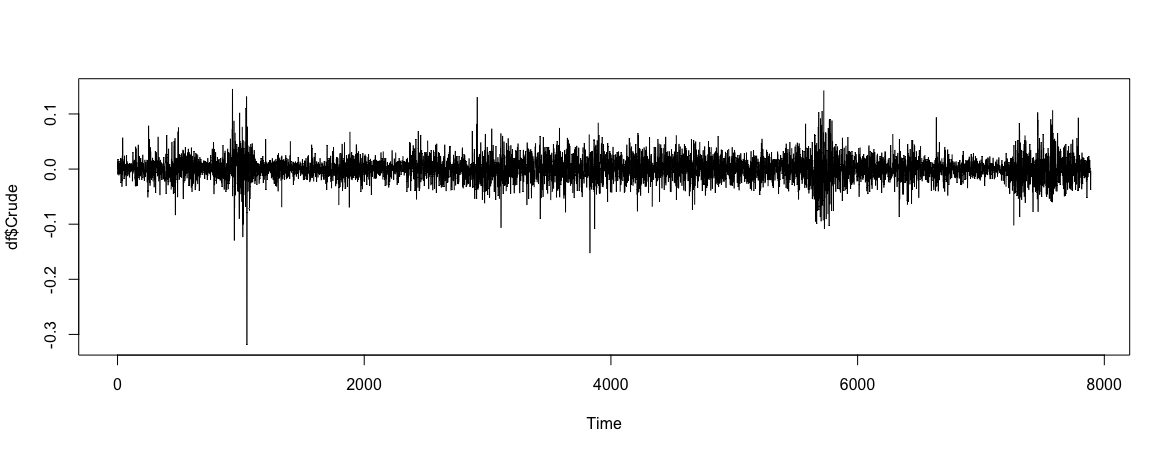
\includegraphics[width=1.0\textwidth]{ts_crude.png}
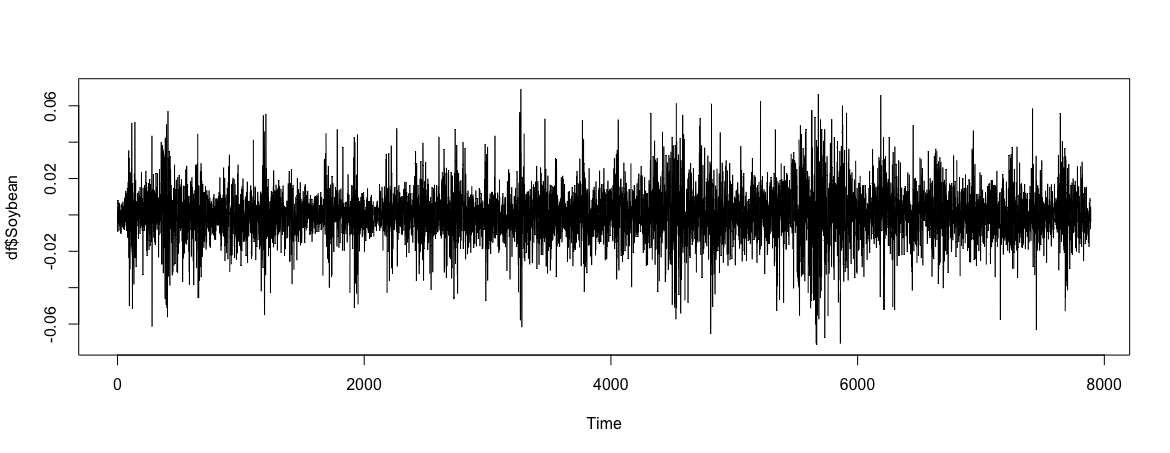
\includegraphics[width=1.0\textwidth]{ts_soybean.png}
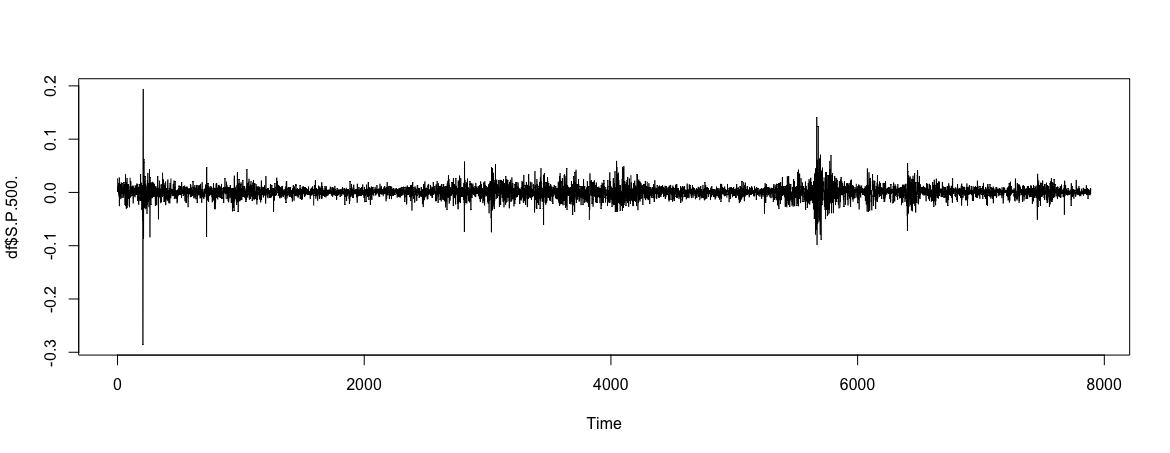
\includegraphics[width=1.0\textwidth]{ts_sp500.png}
\caption{\label{ts} Time Series plots for Crude, Soybean and S$\&$P500}
\end{figure}

\begin{figure}
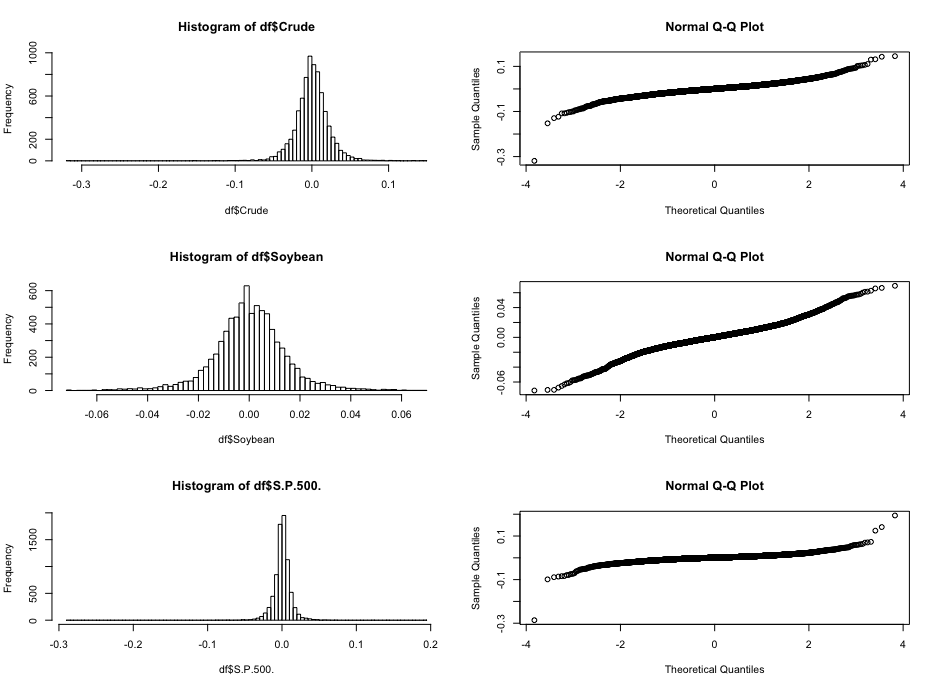
\includegraphics[width=1.0\textwidth]{histqq.png}
\caption{\label{histqq} Histograms and Q-Q plots for Crude, Soybean and S$\&$P500}
\end{figure}

\subsection{Methodology}

Following section 5 in chapter 10 of Politis (2015) \cite{Politis2015} we focus on the simple problem of one-step ahead prediction. To be simulate the performance of a real world production system that produces volatility forecasts, we use the entire length of the daily returns time series minus the most recent date. Consequently for all 5 futures contracts we're forecasting the volatility on the last day of available data - April 20, 2017. In order to replicate the results from Tables 10.3 and 10.5 in chapter 10 we simply plug in our time series into the provided R functions that generate those results. To calculate the entries in table \ref{results} we divide the forecasted returns from our baseline predictor (1) with the forecasted returns for our chosen method. The methods we consider are exponential smoothing (with the discount factor $\delta$ chosen by CV), GARCH(1,1) with both normal and $t$ distribution errors and the simple and exponential NoVaS predictors. We make a number of assumptions about the distribution of the data that we empirically check but for brevity do not display in this report. Lastly, due to the reasonably large sample size of the time series there were computational intractability issues when trying to do MLE for GARCH modeling. In these cases we chose to update the dataset parameters every $n/30$ days so that the GARCH models would actually converge in a reasonable amount of time.   

\subsubsection{Mean Absolute Deviation (MAD) prediction}

As per Politis (2015) \cite{Politis2015} we focus on Mean Absolute Deviation (MAD) of prediction as the author observes that a large discrepancy exists between the performance measures of Mean Squared Error (MSE) and MAD. The argument made as to why this is the case is due to the fact that the financial returns data seems to finite variance but infinite fourth moment. We empirically check this fact for our data by plotting the $VAR_k(Y)$ and $KURT_k(Y)$ the sample variance and kurtosis of dataset $Y$ up to time $k$ i.e. $\{Y_1,\dots,Y_k\}$. We plot the results for these values as a function of $k$ and find in figure \ref{kurtvar} that indeed for the S$\&$P500 data the sample variance seems to eventually converge whereas the sample kurtosis seems to diverge. Therefore it is not surprising that the $L_2$ measure of prediction performance is likely to yield suboptimal results as the MSE of predicting $Y_{n+1}^2$ is essentially a fourth moment and the data suggests that these maybe infinite. 

Thus, we focus on the objective of the $L_1$-optimal prediction where the optimal predictor is the conditional median. Under the ARCH(p) model (3) the $L_1$-optimal predictor of $Y_{n+1}^2$ is given by

\begin{equation}
Median(Y_{n+1}^2|F_n) = a + \sum_{i=1}^p a_i Y_{n+1-i}^2 Median(Z_{n+1}^2)
\end{equation}

Having already chosen the NoVaS parameters we can rearrange equation (7) to yield:

\begin{equation}
Y_t = \frac{W_{t,a}}{\sqrtsign{1-a_0 W_{t,a}^2}} \sqrtsign{\alpha s_{t-1}^2 + a_{0} Y_{t}^2 + \sum_{i=1}^p a_i Y_{t-i}^2} \hspace{0.2cm} \text{for} \hspace{0.2cm} t = p+1,\dots, n
\end{equation}

Hence we can write the predictive distribution (given $F_n$) of $g(Y_{n+1})$ (where $g(x)=x^2$ is the function of interest for volatility prediction) is identical to the distribution of the random variable

\begin{equation}
g(A_n \frac{W}{\sqrtsign{1 - a_0W^2}})
\end{equation}

where $A_n = \sqrtsign{\alpha s_{t-1}^2 + a_{0} Y_{t}^2 + \sum_{i=1}^p a_i Y_{t-i}^2}$ is treated as a constant given the past $F_n$. Thus as mentioned above, the best (in an $L_1$ sense) prediction of $g(Y_{n+1})$ given $F_n$ is given by the median of the conditional distribution of $g(Y_{n+1})$

\begin{equation}
\widehat{g(Y_{n+1})} \coloneqq Median(g(A_n \frac{W_{n+1,a}}{\sqrtsign{1 - a_0W_{n+1,a}^2}})|F_{n})
\end{equation}

Focusing on volatility prediction and the function $g(x)=x^2$ yields the NoVaS predictor

\begin{equation}
\widehat{Y_{n+1}^2} = \mu_{2}A_{n}^2
\end{equation}

where

\begin{equation}
\mu_{2} = Median(\frac{W_{n+1,a}}{1 - a_0W_{n+1,a}^2})|F_{n})
\end{equation}

Making the assumption that the NoVaS series $\{W_{t,a}\}$ appears to be uncorrelated (which we briefly checked but do not display here) we can estimate $\mu_2$ by the sample median

\begin{equation}
\hat{\mu_{2}} = Median\{\frac{W_{n+1,a}}{1 - a_0W_{n+1,a}^2}; t=p+1,p+2,\dots,n\}
\end{equation}

and therefore we can predict $Y_{n+1}^2$ by $\hat{\mu_{2}}A_{n}^2$.

\begin{figure}
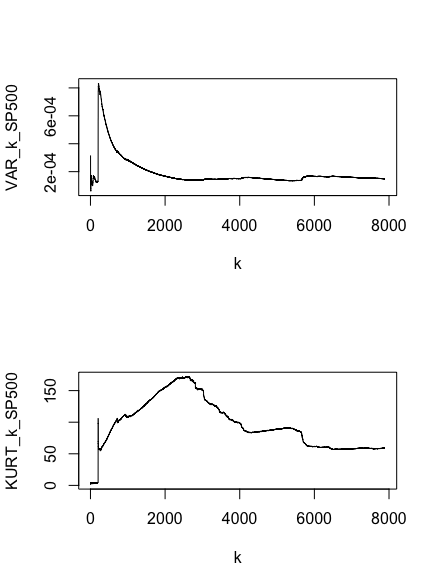
\includegraphics[width=1.0\textwidth]{kurtvar.png}
\caption{\label{kurtvar} (S$\&$P500) Plot of $VAR_k(Y)$ as a function of $k$ and plot of $KURT_k(Y)$ as a function of $k$}
\end{figure}

\subsection{Prediction Results}

\begin{table}[ht]

\begin{tabular}{ |p{6cm}||p{1cm}|p{1cm}|p{1.4cm}|p{1.3cm}|p{1.2cm}|p{2cm}|}
 \hline
 Method & Crude & Gold & Soybean & S$\&$P500 & US10yr & DollarIndex\\
 \hline
 Exponential Smoothing with CV   & 1.126  & 1.091 & 0.973 & 1.213 & 1.086 & 1.038\\
 GARCH(1,1) with Normal errors  & 0.941 & 0.906 & 0.892 & 1.021 & 0.954 & 0.881\\
 GARCH(1,1) with $t$ errors  & 0.917  & 0.928 & 0.906 & 0.983 & 0.937 & 0.913\\
 Simple NoVaS  & 0.847  & 0.819 & 0.804 & 0.864 & 0.781 & 0.845\\
 Exponential NoVaS  & 0.863  & 0.759 & 0.771 & 0.838 & 0.817 & 0.837\\
 \hline
\end{tabular}
\caption{\label{results} Entries give the empirical Mean Absolute Deviation (MAD) of prediction of squared returns relative to benchmark; note that the MAD of prediction achieved by the benchmark was 0.0004492945, 0.0001004134, 0.0001975508, 0.0001454869, 1.510072e-05, 2.926186e-05 for Crude, Gold, Soybean, S$\&$P500, US10yr and DollarIndex respectively}
\end{table}

\begin{figure}[ht]
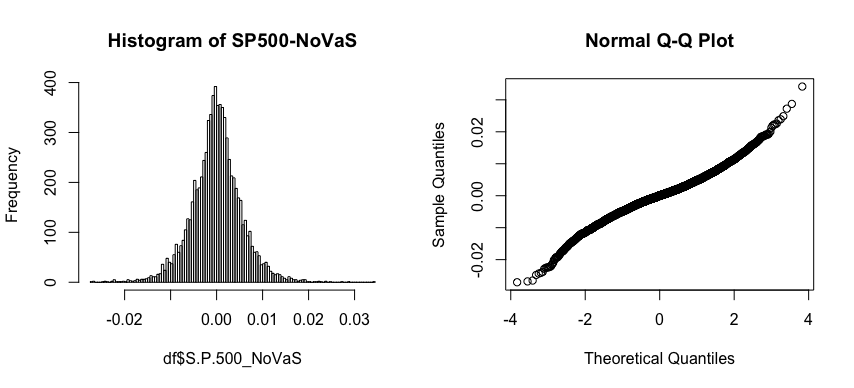
\includegraphics[width=1.0\textwidth]{sp500_novas.png}
\caption{\label{sp500_novas} (S$\&$P500) Histogram and Q-Q plot of transformed NoVaS time series}
\end{figure}

The results in table \ref{results} provide the empirical MAD of prediction of squared returns relative to the benchmark. Due to implementation errors it's possible that not all of the individual entries are correct, however we wish to highlight that the overall trend is quite clear. As expected, the model-free prediction NoVaS methods outperform the exponential smoothing and GARCH(1,1) methods. This is consistent with results shown in Chapter 10 in Politis (2015) \cite{Politis2015}. Note that the results are not significantly better largely because we chose to implement the most basic least optimized version of NoVaS in order to argue that even in this baseline NoVaS case, one can outperform GARCH(1,1) for volatility prediction.

Figure \ref{sp500_novas} shows the histogram and normal Q-Q plot of the simple NoVaS transformed time series and we note that while it does not appear to be exactly normal, in comparison to the original data $\{Y_t\}$ displayed in figure \ref{histqq} it is clear that the transformation normalizes and variance-stabilizes the data.

\section{Conclusion}
In this project, we were able to show that the model-free approach outperforms the model-based approach in the context of volatility prediction. We closely followed Chapter 10 in Politis (2015) \cite{Politis2015} and were able to find similar results in the most simple case. The literature on volatility prediction is quite large and we refer the interested reader to Poon and Granger (2003) \cite{PoonGranger2003} and Andersen et. al (2006) \cite{Andersen2006} for comprehensive reviews of the subject. For a more detailed treatment of NoVaS we refer the reader to Politis (2007) \cite{Politis2007} and Politis and Thomakos (2012) \cite{Politis2012}. 

Finally, we'd like to note some of the shortcomings of our investigation and further avenues of exploration. The most significant shortcoming of our investigation was the time intensive nature of attempting to accurately run all our methods across our six chosen futures time series. As a result, we were unable to implement the basic model-free bootstrap algorithm for prediction intervals. Our initial results in doing so yielded unreasonably large (in this author's opinion) prediction intervals and the effort was abandoned in the interest of time - we aim to implement these in the coming months. We note that the model-free approach is unreasonably suited to using the bootstrap because of it's emphasis on observed values as opposed to estimated parameters. Lastly, there were a number of extensions to NoVaS such as generalized Simple/Exponential NoVaS and Time-Varying NoVaS that were optimized to the task of volatility prediction. Once again in the interest of time these were not explored but the aim is to do so in the near future. Based on our current results we expect that we'll see significant improvement with regard to our naive baseline once these are implemented.
\vspace{-0.7cm}
\nocite{*}
\bibliographystyle{plain}
\bibliography{newbib_thesis}
\end{document}